% \documentclass[]{IEEEphot}
\documentclass[12pt,a4paper]{article}
% \jmonth{April}
% \pubyear{2023}

\newtheorem{theorem}{Theorem}
\newtheorem{lemma}{Lemma}
\usepackage{hyperref}
% \usepackage{graphicx,caption}
\usepackage{graphicx}
\usepackage{float}
\usepackage{adjustbox}
\usepackage{amsmath}
\usepackage{mathtools} 
\usepackage{algorithm}
\usepackage{algpseudocode}

\begin{document}

\title{Detection of circular trade using Node2Vec and DBScan}

\author{Dinesh Avula\\CS20BTECH11005
\and Ayush Jha\\CS20BTECH11006 \and Vaibhav Chhabra\\AI20BTECH11022 \and Yuvraj Singh Shekhawat\\CS20BTECH11057 \and
Rohan Atkurkar\\CS20BTECH11041 }


\maketitle

\section{Problem statement}
The goal of this project is to detect fraudulent circular trading activities in a transaction dataset that involves buyers, sellers, and their transactions. To achieve this goal, we first convert the dataset into a directed unweighted graph and then into an undirected weighted graph. The weights of the graph are proportional to the number of 2 and 3 cycles, which helps in identifying fraudulent circular trading patterns. The graph is then converted to vectors using Node2Vec, which helps in detecting the similarity between different nodes. Finally, we apply the DBScan algorithm to identify clusters of fraudulent people involved in circular trading. This approach enables us to detect and prevent fraudulent activities in the transaction dataset,

\section{Background}
\subsection{Circular Trading}
A fraudulent circular trade, also known as a round-trip transaction, occurs when two or more parties engage in a series of trades or transactions that appear legitimate but are designed to manipulate financial statements and deceive investors or other stakeholders. In a typical circular trade scheme, one company sells goods or services to another company, and that second company, in turn, sells goods or services back to the first company. The cycle then repeats itself, often involving multiple companies or intermediaries, creating the appearance of legitimate transactions and financial activity. 

\subsection{Node2Vec}
Node2Vec is a graph embedding algorithm that learns low-dimensional vector representations (embeddings) of nodes in a graph. It is based on the idea of generating random walks on the graph and optimizing a likelihood function to ensure that nodes that appear in similar contexts in these walks end up with similar embeddings. Node2Vec balances between the breadth-first search (BFS) and depth-first search (DFS) strategies to generate random walks that capture both local and global structures of the graph.
\subsection{DBSCAN}
DBSCAN is a clustering algorithm that groups together points that are close to each other and identifies outliers that are far from any cluster.
The algorithm has two important hyperparameters:
\begin{enumerate}
    \item eps: It specifies the maximum distance between two points for them to be considered as in the same neighborhood.
    \item  min-samples: It specifies the minimum number of points required to form a dense region. Points that are not part of any dense region are considered as noise.
\end{enumerate}



\section{Description of dataset}
\begin{itemize}
    \item We have total of 130535 transactions each containing seller id, buyer id and transaction value. 
    \item There are 799 unique ids which means there are 799 dealers.
    \item There are total of 130535 transactions but most of them are between same set of dealers. There are 5358 transactions between different dealers.
    \item Below is a small sample of data from our dataset.
\end{itemize}
\begin{figure}[H]
\centering
\label{fig:CP }
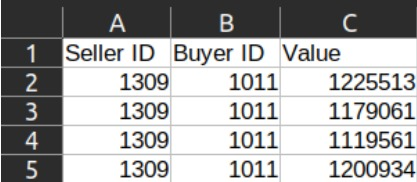
\includegraphics[width=10cm]{DatasetSample.png}
\end{figure}

\section{Naive Solutions}
While the traditional method of detecting fraudulent circular trading involves converting the transaction dataset to a directed weighted multigraph and running cycle detection graph algorithms, this approach may not be feasible in real-world scenarios. The main issue with this method is its scalability, as the sheer size of the transaction data can overwhelm the graph algorithms, making it difficult to detect fraudulent activities. 
As the number of transactions increases, the graph algorithms require more computational power and storage space, which can result in slow performance and longer processing times. This makes the traditional approach impractical for detecting fraudulent circular trading in large datasets, which is a common scenario in the business world.

\section{Algorithm}
\subsection{Initial Preprocessing Steps}
The  following is done to solve the problem statement : 
\begin{enumerate}
    \item The first step is to preprocess, it involves converting the data from CSV format to NumPy arrays, which can then be used for further analysis.
    \item The graph is constructed as a directed, unweighted graph, with each edge representing a transaction between two parties. For each transaction, a frequency vector is maintained, which keeps track of the number of times that particular transaction has occurred.
    \item Once the frequency vector is constructed, the edge representing the transaction is added to the directed graph. 
\end{enumerate}

\subsection{Converting to undirected Graph}
Now we have to convert this graph into an edge weighted undirected graph.

\begin{figure}[H]
\centering
\label{fig:3cycle}
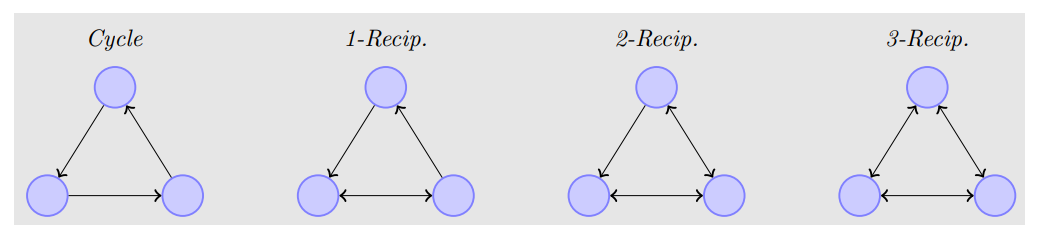
\includegraphics[width=12cm]{3-cycle.png}
\end{figure}

In order to accomplish that we follow the steps given in the research paper Commuinty detection in Networks : 
\begin{enumerate}
    \item Initially, the vectors $r_0, r_1, r_2,$ and $r_3$ are set to  0 based on the paper and Figure \ref{fig:3cycle} represents them. $r_0$ represents the 3-cycles that have no reciprocal edges, $r_1$ represents the 3-cycles that have one reciprocal edge, $r_2$ represents the 3-cycles that have two reciprocal edges, and $r_3$ represents the 3-cycles that have three reciprocal edges.
    \item Next, we iterate over the edges of the graph and count the number of 3-cycles with reciprocal edges in the directed graph. The corresponding bit vectors ($r_0$, $r_1$, $r_2$, $r_3$) are set to 1 based on the number of reciprocal edges found in the cycle.
    \item Then using these indicating bit vectors $r_0, r_1, r_2,$ and $r_3$, the weight of each edge in the directed graph is calculated based on the formula $$ w = max \{ 4 \ast r_3, 3\ast r_2, 3\ast r_1, 2\ast r_0, 1 \}$$
    \item These weights are multiplied by the scaled frequency vectors (which indicate the no. of transactions between those two nodes).
    \item While adding the edges to the final undirected graph, in case of a double edge the maximum of both the weights is chosen as the weight and the newly constructed graph is returned. 
\end{enumerate}

\subsection{Node2Vec}
    The Node2Vec algorithm is used to create embeddings of nodes based on their weights calculated from the previous algorithm. The following hyperparameters are used:
    \begin{enumerate}
    \item $dimensions=64$, 
    \item $\text{walk-length}=10 $, 
    \item $\text{num-walks}=200$, 
    \item $p=1$, 
    \item $q=1/2$, 
\end{enumerate}

\subsection{DBSCAN}
    The embeddings obtained from Node2Vec are used as input for the DBSCAN algorithm to identify clusters. The elbow method is used to obtain the optimal value of eps hyperparameter in DBSCAN. 
    \begin{figure}[H]
    \centering
    \label{fig:eps}
    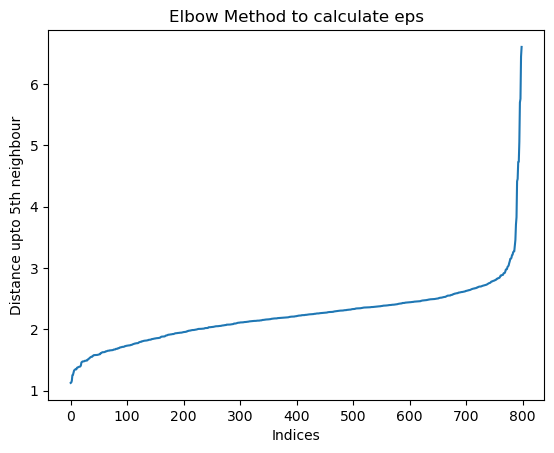
\includegraphics[width=12cm]{EPS.png}
    \end{figure}
    In the above figure we obtain a sudden rate of change of the distance value at around 1.5, hence the $eps=1.5$ 
    The algorithm uses the following hyperparameters: 
    \begin{enumerate}
    \item $eps = 1.5$ obtained eperimentally using the elbow method as seen in figure \ref{fig:eps}, 
    \item $\text{min-samples} = 5 $ chosen parameter
\end{enumerate}
\section{Results}
    \begin{figure}[H]
    \centering
    \label{fig:woclusters}
    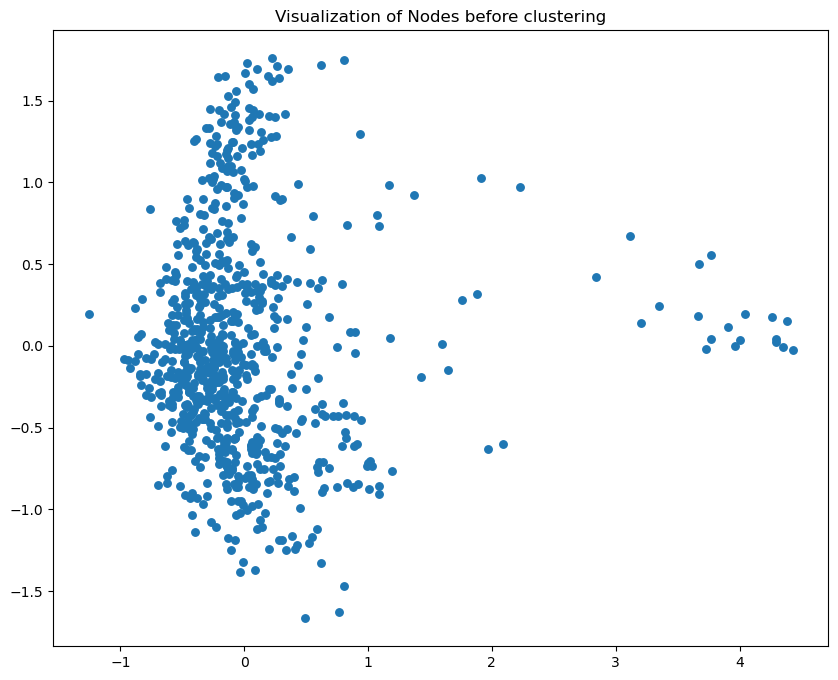
\includegraphics[width=12cm]{woclustering.png}
    \end{figure}
    The above figure \ref{fig:woclusters} represents all of the node embeddings generated by Node2Vec and their transformation on 2-dimensional space using PCA.
    \begin{figure}[H]
    \centering
    \label{fig:clusters}
    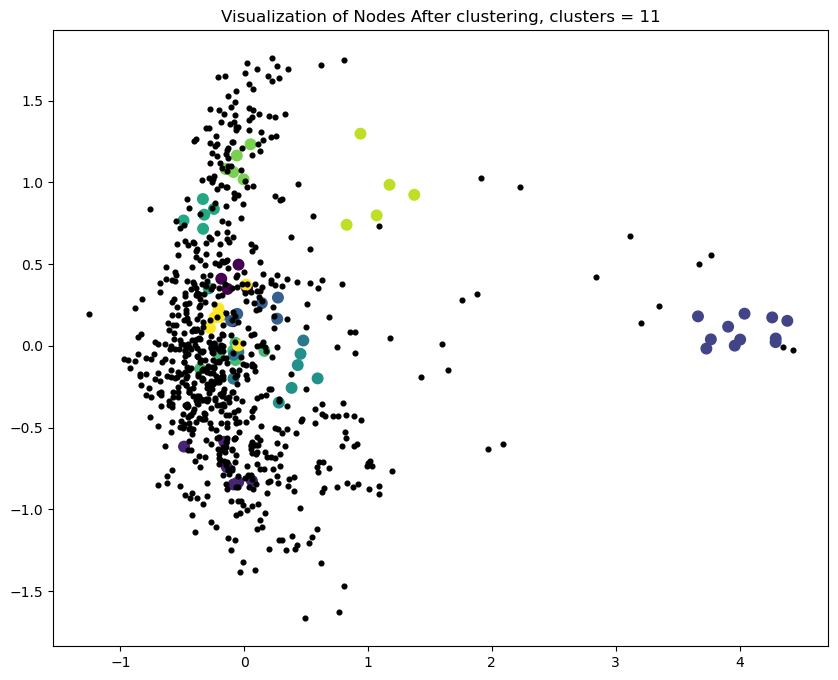
\includegraphics[width=12cm]{clustering.png}
    \end{figure}
   In figure \ref{fig:clusters}, the colored dots represent the vectors clustered by DBSCAN, which indicates that they could be fraudulent points. The black dots were classified as "noise points" by DBSCAN. To display the original node embeddings in 2D space, PCA was used again. The algorithm was able to detect 11 clusters of nodes with an average of 5 to 6 points per cluster, indicating that we chose the appropriate set of hyperparameters after continuous experimentation.
\section{Conclusions}
In this project, we applied an approach to identify fraudlent groups of users from a finance dataset using a combination of graph-based and clustering techniques. We first computed the weights of edges in the graph based on the number of 3-cycles and reciprocity, and then generated node embeddings using the Node2Vec algorithm. Finally, we applied the DBSCAN algorithm on the embeddings to identify clusters of users.

The results showed that the approach used was able to identify meaningful clusters of users, which could then be used for further investigation. However, we also noted that the performance of the approach could be affected by the choice of hyperparameters.



\end{document}
